% 135-31(135쪽) — 어느 두 직선도 평행하지 않고 어느 세 직선도 한 점에서 만나지 않게 그은 직선 3개(a_3=7 의 예시 그림).
% 스캔 화질이 낮아 TikZ 로 다시 그림. 원문에 라벨이 없으므로 라벨을 넣지 않고, 나뉜 영역의 개수도 표시하지 않는다.
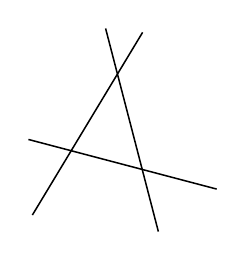
\begin{tikzpicture}[scale=1, line width=0.55pt]
  \draw (1.19,2.61) -- (1.86,0.03);
  \draw (1.66,2.56) -- (0.26,0.24);
  \draw (0.21,1.20) -- (2.60,0.57);
\end{tikzpicture}
